% !TeX root = 机械设计.tex
% ============================================================
%  第二章 机械零件的强度
%  来源：教材/机械设计《机械原理与机械设计（下）》读书笔记
%  说明：正文表述与公式均沿用原文，仅作版式与环境归类
% ============================================================
\chapter{机械零件的强度}
\label{chap:机械零件的强度}

\section{载荷与应力的分类}
\label{sec:载荷与应力的分类}

\subsection{载荷的分类}
\label{subsec:载荷的分类}

\begin{definition}[静载荷]
\label{def:静载荷}
\textbf{静载荷}：载荷的大小和方向不随时间变化或变化缓慢的载荷。
\end{definition}

\begin{definition}[变载荷]
\label{def:变载荷}
\textbf{变载荷}：载荷的大小和方向随时间变化的载荷。变载荷可分为
\begin{enumerate}
	\item 循环变载荷：
	\begin{enumerate}
		\item 稳定循环载荷；
		\item 不稳定循环载荷。
	\end{enumerate}
	\item 随机变载荷。
\end{enumerate}
\end{definition}

\subsection{应力的分类}
\label{subsec:应力的分类}

\begin{definition}[静应力]
\label{def:静应力}
\textbf{静应力}：不随时间变化或变化缓慢的应力，其随时间的变化规律如图~\ref{fig:静应力} 所示。
\end{definition}

\begin{figure}[H]
\centering
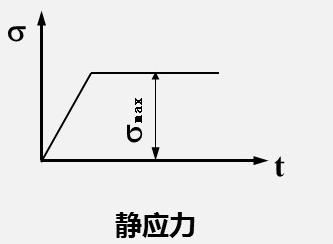
\includegraphics[width=0.52\textwidth]{Figure/静应力.png}
\caption{静应力}
\label{fig:静应力}
\end{figure}

\begin{definition}[变应力]
\label{def:变应力}
\textbf{变应力}：随时间变化的应力，可分为
\begin{enumerate}
	\item \textbf{不稳定变应力}：
	\begin{enumerate}
		\item 规律性不稳定变应力，如图~\ref{fig:规律性不稳定变应力} 所示；
		\item 随机变应力，如图~\ref{fig:随机变应力} 所示。
	\end{enumerate}
	\item \textbf{稳定循环变应力}：
	\begin{enumerate}
		\item 非对称循环变应力，如图~\ref{fig:非对称循环变应力} 所示；
		\item 脉动循环变应力，如图~\ref{fig:脉动循环变应力} 所示；
		\item 对称循环变应力，如图~\ref{fig:对称循环变应力} 所示。
	\end{enumerate}
\end{enumerate}
\end{definition}

\begin{figure}[H]
\centering
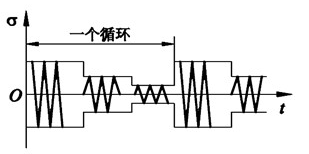
\includegraphics[width=0.6\textwidth]{Figure/规律性不稳定变应力.png}
\caption{规律性不稳定变应力}
\label{fig:规律性不稳定变应力}
\end{figure}

\begin{figure}[H]
\centering
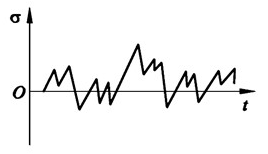
\includegraphics[width=0.55\textwidth]{Figure/随机变应力.png}
\caption{随机变应力}
\label{fig:随机变应力}
\end{figure}

\begin{figure}[H]
\centering
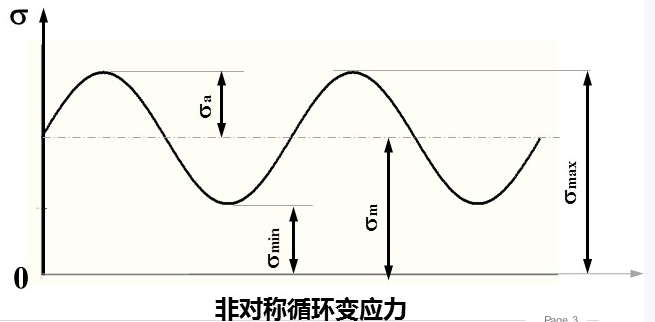
\includegraphics[width=0.72\textwidth]{Figure/非对称循环变应力.png}
\caption{非对称循环变应力}
\label{fig:非对称循环变应力}
\end{figure}

\begin{figure}[H]
\centering
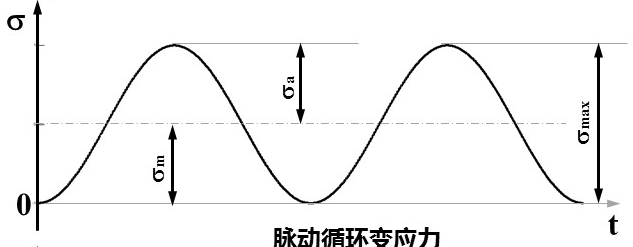
\includegraphics[width=0.68\textwidth]{Figure/脉动循环变应力.png}
\caption{脉动循环变应力}
\label{fig:脉动循环变应力}
\end{figure}

\begin{figure}[H]
\centering
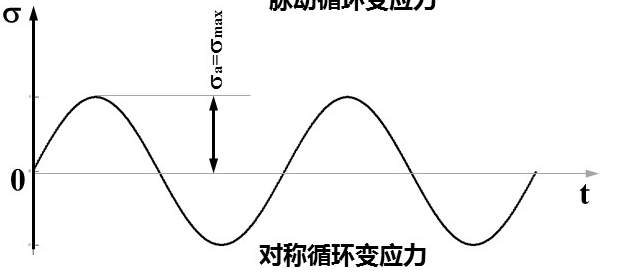
\includegraphics[width=0.68\textwidth]{Figure/对称循环变应力.png}
\caption{对称循环变应力}
\label{fig:对称循环变应力}
\end{figure}

\subsection{稳定循环变应力的基本参数}
\label{subsec:稳定循环变应力参数}

稳定循环变应力的基本参数包括最大应力 $\sigma_{\max}$、最小应力 $\sigma_{\min}$、平均应力 $\sigma_m$ 和应力幅 $\sigma_a$，其相互关系如下。

\textbf{（1）平均应力}是指循环变应力中静应力分量的部分，其值为
\begin{equation}
	\sigma_m = \frac{\sigma_{\max}+\sigma_{\min}}{2}
	\label{eq:强度:平均应力}
\end{equation}

\textbf{（2）应力幅}是指循环变应力中变动应力分量的部分，其值为
\begin{equation}
	\sigma_a = \frac{\sigma_{\max}-\sigma_{\min}}{2}
	\label{eq:强度:应力幅}
\end{equation}

\textbf{（3）应力循环特性（循环比）}是指最小应力与最大应力之比，即
\begin{equation}
	\gamma = \frac{\sigma_{\min}}{\sigma_{\max}}, \qquad -1 < \gamma < +1
	\label{eq:强度:循环特性}
\end{equation}

\begin{keybox}[脉动循环与对称循环]
脉动循环变应力：$\gamma=\dfrac{\sigma_{\min}}{\sigma_{\max}}=0$（$\sigma_{\min}=0$）；
对称循环变应力：$\gamma=\dfrac{\sigma_{\min}}{\sigma_{\max}}=-1$（$\sigma_{\max}=-\sigma_{\min}$）。
\end{keybox}
